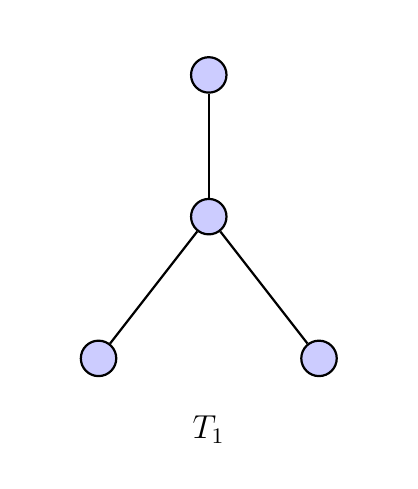
\begin{tikzpicture}[
  baseline=0pt,
  scale=1,
  vnode/.style={circle, draw=black, fill=blue!20, thick, inner sep=0pt, minimum size=4.5mm},
  edge/.style={thick, draw=black}
]
  \useasboundingbox (-2.3,-3.1) rectangle (2.3,2.4);

  % 4 vértices (Estrella / Tridente)
  \node[vnode] (v1) at (0, 1.8) {};     % Vértice superior
  \node[vnode] (v2) at (0, 0.0) {};     % Vértice central
  \node[vnode] (v3) at (-1.4, -1.8) {}; % Vértice inferior izq
  \node[vnode] (v4) at (1.4, -1.8) {};  % Vértice inferior der

  % Aristas
  \draw[edge] (v2) -- (v1);
  \draw[edge] (v2) -- (v3);
  \draw[edge] (v2) -- (v4);

  % Etiqueta
  \node[font=\large] at (0,-2.7) {$T_1$};
\end{tikzpicture}
